\documentclass{beamer}

\usepackage{url}

\newcommand\vs{\vspace{\baselineskip}}

\newcommand\titlecite{
{\em Of all natural systems, living matter preserves inscribed in its organization the largest amount of its own past history .... no other system is better}
 aufgehoben:
{\em constantly abolished and simultaneously preserved.}
\cite{PaulingZuckerkandl63}}

\newcommand\presentation[1]{ \section*{PRESENTATION: #1} }



% workaround for beamer bug
\providecommand\thispdfpagelabel[1]{}  % workaround

% presentation
\mode<presentation>
{
  \usetheme{Warsaw}
  % or ...

  \setbeamercovered{transparent}
  % or whatever (possibly just delete it)
}


\usepackage[english]{babel}
% or whatever

\usepackage[latin1]{inputenc}
% or whatever

\usepackage{times}
\usepackage[T1]{fontenc}
% Or whatever. Note that the encoding and the font should match. If T1
% does not look nice, try deleting the line with the fontenc.


\title[MCMC] % (optional, use only with long paper titles)
{Markov Chain Monte Carlo}

\subtitle
{Metropolis-Hastings and related algorithms} % (optional)

\author% [Holmes] (optional, use only with lots of authors)
{I.~Holmes} % \inst{1} \and S.~Another\inst{2}
% - Use the \inst{?} command only if the authors have different
%   affiliation.

\institute[University of California, Berkeley] % (optional, but mostly needed)
{
%  \inst{1}%
  Department of Bioengineering\\
  University of California, Berkeley}
% - Use the \inst command only if there are several affiliations.
% - Keep it simple, no one is interested in your street address.

\date%[Short Occasion] % (optional)
{Spring semester}

\subject{Talks}
% This is only inserted into the PDF information catalog. Can be left
% out. 



% If you have a file called "university-logo-filename.xxx", where xxx
% is a graphic format that can be processed by latex or pdflatex,
% resp., then you can add a logo as follows:

% \pgfdeclareimage[height=0.5cm]{university-logo}{university-logo-filename}
% \logo{\pgfuseimage{university-logo}}



% Delete this, if you do not want the table of contents to pop up at
% the beginning of each subsection:
\AtBeginSubsection[]
{
  \begin{frame}<beamer>{Outline}
    \tableofcontents[currentsection,currentsubsection]
  \end{frame}
}


% If you wish to uncover everything in a step-wise fashion, uncomment
% the following command: 

%\beamerdefaultoverlayspecification{<+->}


\begin{document}

\begin{frame}
  \titlepage
\end{frame}

\begin{frame}{Outline}
  \tableofcontents
  % You might wish to add the option [pausesections]
\end{frame}

\section{Conjugate prior distributions}

\begin{frame}{Motivation}

\itemb
\item $P(\theta|x)$ and $P(\theta)$ are \alert{conjugate} if the posterior $P(\theta|x)$ is of the same family as the prior $P(\theta)$
\[
P(\theta|x) = \frac{P(x|\theta) P(\theta)}{P(x)} = \frac{P(x|\theta) P(\theta)}{\int P(x,\theta') d\theta'}
\]
\item The denominator is $P(x)$, the \alert{Bayesian evidence}, which does not depend on $\theta$.
\item The dependence of $P(\theta|x)$ on $\theta$ is same as that of $P(x|\theta)P(\theta)$,
but to get a normalized form for $P(\theta|x)$, we need to integrate out $\theta$ to find the evidence $P(x)$.
\item The parameters of the conjugate prior distribution are called \alert{hyperparameters}.
\iteme

\end{frame}

\subsection{Gamma distribution}

\begin{frame}{Gamma distribution}

\itemb
\item Exponential, Poisson, Gamma distributions
 \itemb
 \item Exponential distribution: pdf for time to first event, $T$, given that mean event rate is $\mu$
\[
P(T|\mu) = \mu \exp(-\mu T)
\]
 \item Poisson: probability distribution of number of events, $n$, in time $T$, given that mean event rate is $\mu$
\[
P(n|\mu) = \frac{(\mu T)^n \exp(-\mu T)}{n!}
\]
(NB exponential distribution can be obtained by setting $n=0$ and differentiating w.r.t. $T$)
\iteme
\iteme


\end{frame}


\begin{frame}{Gamma distribution}

\itemb
 \item Poisson
\[
P(n|\mu) = \frac{(\mu T)^n \exp(-\mu T)}{n!}
\]
 \item Gamma, conjugate to Poisson. \\
Shape parameter $\alpha$, rate parameter $\beta$.
\[
P(\mu|\alpha,\beta) = \frac{\mu^{\alpha-1} \beta^\alpha \exp(-\mu \beta)}{\Gamma(\alpha)}
\]
where $\Gamma$ is the \alert{gamma function}
\[
\Gamma(\alpha) = \int_0^{\infty} (\mu\beta)^{\alpha-1} \exp(-\mu \beta) d(\mu \beta)
\]
\iteme


\end{frame}


\begin{frame}{Gamma function}

Changing variables in the gamma function integral
\[
\Gamma(z) = \int_{u=0}^\infty u^{z-1} \exp(-u) du
\]
Clearly $\Gamma(1)=1$. Integrating by parts for positive integer $z$,
\begin{eqnarray*}
\Gamma(z+1) & = & \int_{u=0}^\infty u^z \exp(-u) du \\
& = & \left[ -u^z \exp(-u) \right]_{u=0}^\infty + z \Gamma(z) \\
& = & z!
\end{eqnarray*}


\end{frame}

\begin{frame}{Gamma distribution}

  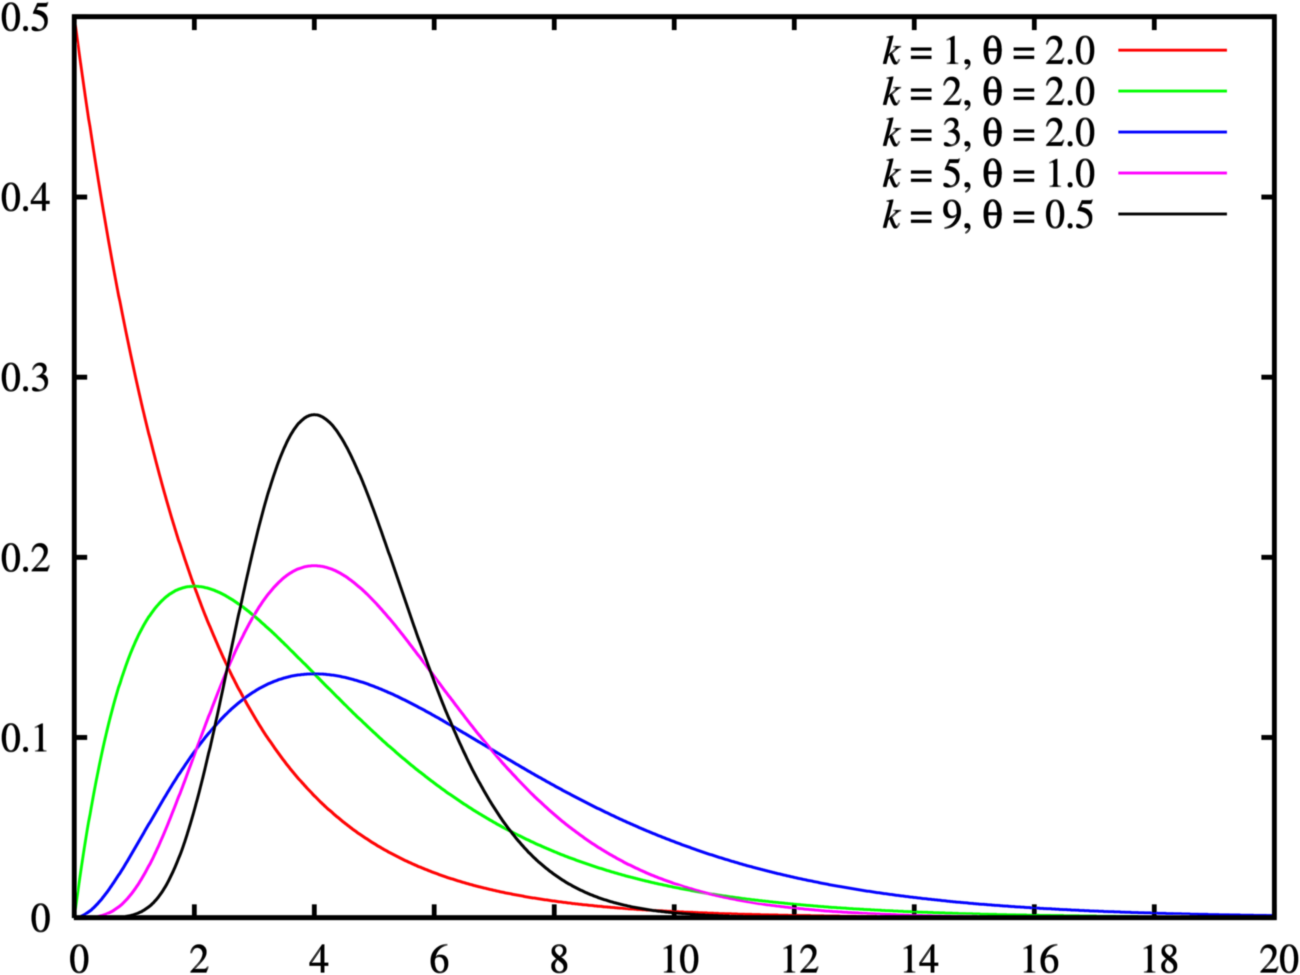
\includegraphics[width=.6\textwidth]{Gamma_distribution.png}

$k=\alpha$, $\theta = 1/\beta$

$\theta$ is called the scale parameter.

\end{frame}

\begin{frame}{Gamma distribution}

\itemb
 \item Properties of gamma distribution: \\ mean of $\mu$ is $\alpha/\beta$ and variance is $\alpha/\beta^2$.
 \item Conjugacy:
\begin{eqnarray*}
P(n) & = & \frac{\Gamma(\alpha')}{\Gamma(n+1)\Gamma(\alpha)} \frac{T^n \beta^\alpha}{(\beta')^{(\alpha')}} \\
P(\mu|n) & = & \frac{\mu^{\alpha'-1} (\beta')^{\alpha'} \exp(-\mu \beta')}{\Gamma(\alpha')}
\end{eqnarray*}
i.e. posterior for $\mu$ is a gamma distribution with shape $\alpha' = \alpha + n$ and rate $\beta' = \beta + t$.
\item $\alpha$ and $\beta$ are like a {\em pseudocount} and {\em pseudotime}.
\iteme


\end{frame}


\begin{frame}{Gamma distribution}

\itemb
 \item Lengthier derivation:
\begin{eqnarray*}
P(n) & = & \int_{\mu=0}^\infty P(n|\mu) P(\mu) d\mu \\
& = & \int_{\mu=0}^\infty \frac{(\mu T)^n \exp(-\mu T)}{\Gamma(n+1)} \frac{\mu^{\alpha-1} \beta^\alpha \exp(-\mu \beta)}{\Gamma(\alpha)} d\mu \\
& = & \frac{T^n \beta^\alpha}{\Gamma(n+1)\Gamma(\alpha)} \int_{\mu=0}^\infty \mu^{n+\alpha-1} \exp(-\mu (T+\beta)) d\mu \\
& = & \frac{T^n \beta^\alpha}{\Gamma(n+1)\Gamma(\alpha)} \frac{1}{(T+\beta)^{n+\alpha}} \int_{u=0}^\infty u^{n+\alpha-1} \exp(-u) du \\
& = & \frac{\Gamma(\alpha')}{\Gamma(n+1)\Gamma(\alpha)} \frac{T^n \beta^\alpha}{(\beta')^{(\alpha')}}
\end{eqnarray*}
\iteme

\end{frame}

\subsection{Dirichlet distribution}

\begin{frame}{Dirichlet distribution}

\itemb
\item Multinomial, Dirichlet distributions
 \itemb
 \item Multinomial: $K$ possible outcomes, outcome probabilities ${\bf p}$, outcome frequencies ${\bf n}$ in $N=\sum_k n_k$ trials
\[
P({\bf n}|{\bf p}) = \frac{N!}{\prod_k n_k!} \prod_k p_k^{n_k}
\]
\item Conjugate prior: let ${\bf a}$ be a vector of \alert{pseudocounts}, $a_1 \ldots a_k$. The \alert{Dirichlet distribution} for ${\bf p}$ is
\[
P({\bf p}|{\bf a}) = \frac{\prod_i p_i^{a_i-1}}{{\cal B}({\bf a})} \delta \left( \sum_i p_i - 1 \right)
\]
where ${\cal B}()$ is the \alert{type one Dirichlet integral} or the \alert{multinomial beta function}
\[
{\cal B}({\bf a})
= \int \left( \prod_i p_i^{a_i-1} \right) \delta \left( \sum_i p_i - 1 \right) d{\bf p}
= \frac{\prod_k \Gamma(a_k)}{\Gamma(\sum_k a_k)}
\]
\iteme
\iteme

\end{frame}


\begin{frame}{Dirichlet distribution}

\itemb
\item Properties: mean value of $p_k$ is $a_k / \sum_j a_j$. Modal value is $p_k = (a_k-1) / (\sum_j a_j-1)$.
% Variance? See Wikipedia...
 \item Note the relationship between the multinomial coefficient and ${\cal B}$
\[
\frac{N!}{\prod_k n_k!} = \frac{1}{{\cal B}({\bf n}+{\bf 1})} \times \frac{\Gamma(N+1)}{\Gamma(N+K)}
\]
 \item Conjugacy:
\begin{eqnarray*}
P({\bf n}|{\bf a}) & = & \frac{{\cal B}({\bf a}')}{{\cal B}({\bf a})} \frac{N!}{\prod_k n_k!}  \\
P({\bf p}|{\bf n},{\bf a}) & = & \frac{\prod_i p_i^{a'_i-1}}{{\cal B}({\bf a}')} \delta \left( \sum_i p_i - 1 \right)
\end{eqnarray*}
where ${\bf a}' = {\bf a} + {\bf n}$ (hence the name ``pseudocount'').
%  \item Here is a plausibility argument for the normalizing constant of the Dirichlet distribution,
% where Dirichlet-distributed probabilities are obtained by normalising Gamma variates.
% Consider counting $K$ types of event, with independent rates $\mu_k$, Poisson-distributed over unit time interval.
% Two equivalent views for joint likelihood $P({\bf n}|\{\mu_k\})$:
%   \enumb
%   \item product of $K$ Poisson likelihoods, each with mean $\mu_k$
% \[
% P({\bf n}|\{\mu_k\}) = \prod_k P(n_k|\mu_k) = \prod_k \frac{\mu_k^{n_k} \exp(-\mu_k)}{n_k!}
% \]
%   \item product of a Poisson likelihood with mean $\mu = \sum_k \mu_k$ for $N$, the total number of events,
% and a multinomial likelihood for the $n_k$ conditional on $N$, with probabilities $p_k = \mu_k / \mu$.
% \[
% P({\bf n}|\mu,{\bf p}) = P(N|\mu) P({\bf n}|{\bf p},N)
% = \frac{\mu^N \exp(-\mu)}{N!} \times \frac{N!}{\prod_k n_k!} \prod_k p_k^{n_k}
% \]
%   \enume
%  \item Note that these are identical. The plausibility argument is that we can similarly equate the posterior distributions, as follows.
%  \item Suppose that we have flat priors $P(\mu_k)=\epsilon$.
% (In fact this is only normalised if $\epsilon$ is vanishingly small or $\mu_k$ is bounded, but let's not worry about this too much for now.)
%  \item Each $\mu_k$ has a gamma posterior with shape $n_k+1$ and scale $1$. Thus joint posterior for the $\{\mu_k\}$ is:
% \begin{eqnarray*}
% P(\{\mu_k\}|{\bf n}) d\mu_1 d\mu_2 \ldots d\mu_k & = & \left( \prod_k P(\mu_k|n_k) \right) d\mu_1 d\mu_2 \ldots d\mu_k \\
% & = & \left( \prod_k \frac{\mu_k^{n_k} \exp(-\mu_k)}{\Gamma(n_k+1)} \right) d\mu_1 d\mu_2 \ldots d\mu_k \\
% & = & \left( \prod_k \frac{(p_k \mu)^{n_k} \exp(-p_k \mu)}{\Gamma(n_k+1)} \right) \left( \delta(\sum_k p_k - 1) . \mu dp_1 . \mu dp_2 \ldots \mu dp_k . d\mu \right) \\
% & = & \frac{\mu^{N+K} \exp(-\mu)}{\Gamma(N+K)} d\mu \times \frac{\Gamma(N+K)}{\prod_k \Gamma(n_k+1)} \left( \prod_k p_k^{n_k} \right) \delta(\sum_k p_k - 1) dp_1 \ldots dp_k \\
% & = & \frac{\mu^{N+K} \exp(-\mu)}{\Gamma(N+K)} d\mu \times \frac{\prod_k p_k^{n_k}}{{\cal B}({\bf n}+{\bf 1})} \delta(\sum_k p_k - 1) dp_1 \ldots dp_k
% \end{eqnarray*}
% % Problem: \mu-term is not a gamma distribution! Normalizing constant should be \Gamma(N+K+1).
% % Not sure how to rigorously justify the expansion $\prod_k d\mu_k = \delta(\sum_k p_k - 1) (\prod_k \mu dp_k) d\mu$
%   \item See how joint posterior for $\{\mu,{\bf p}\}$ can be written as product of Gamma with shape $N+1$ and scale $1$ (for $\mu$)
% and Dirichlet with pseudocounts ${\bf n}+{\bf 1}$ (for ${\bf p}$).
% by setting $p_k = \mu_k / \sum_i \mu_i$, where the $\mu_k$ are Gamma-distributed with scale 1.
% As well as being an equivalent definition of the Dirichlet, this is a common practical way of sampling from a Dirichlet.
 \iteme  

\end{frame}

\begin{frame}{Dirichlet distribution}

\itemb
 \item Special case of \{Multinomial,Dirichlet\} when $K=2$ is \{Binomial,Beta\}, and ${\cal B}$ is the \alert{beta function}.
 \item The following snippets from Mathworld point to a more rigorous solution of the type one Dirichlet integral
  \itemb
  \item The beta integral may be obtained by writing $m!n!$ as a product of gamma functions with integrands $u,v$, transforming to $(x,y)=(\sqrt{u},\sqrt{v})$ and then to polar co-ordinates $(x,y)=r(\cos\theta,\sin\theta)$. This yields
\[
{\cal B}(m+1,n+1) = 2\int_0^{\pi/2} \cos^{2m+1} \theta \sin^{2n+1} \theta d\theta
= \frac{m!n!}{(m+n+1)!}
\]
See {\tt mathworld.wolfram.com/BetaFunction.html}\ for details.
  \item More info on Dirichlet type one integral at {\tt mathworld.wolfram.com/DirichletIntegrals.html}
  \iteme
\iteme

\end{frame}

\begin{frame}{Beta distribution}

  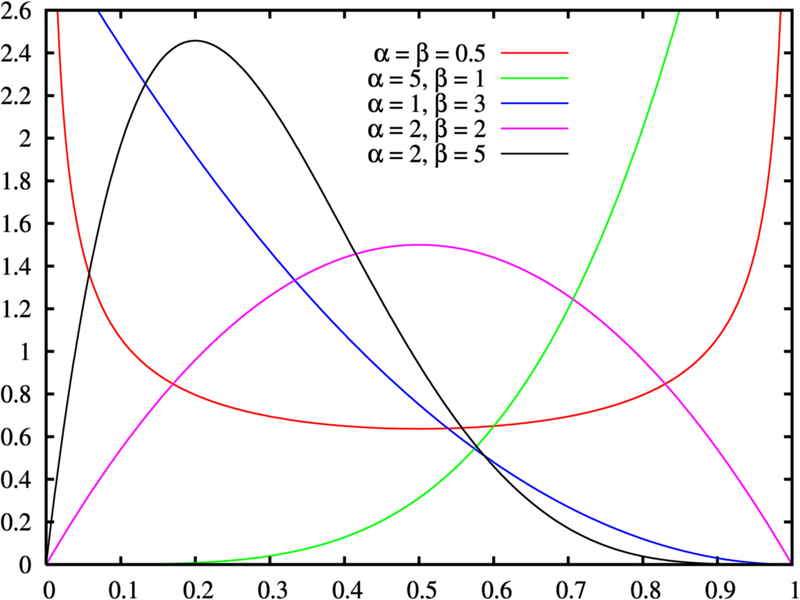
\includegraphics[width=.8\textwidth]{Beta_distribution.png}

\end{frame}

\begin{frame}{Dirichlet distribution}

\itemb
\item
For $K=3$,
the probabilities $(p_x,p_y,p_z)$
satisfy $p_x+p_y+p_z=1$
\item Like 3D points lying on the 2D triangle
with corners at $(0,0,1)$, $(0,1,0)$ and $(1,0,0)$
\iteme

  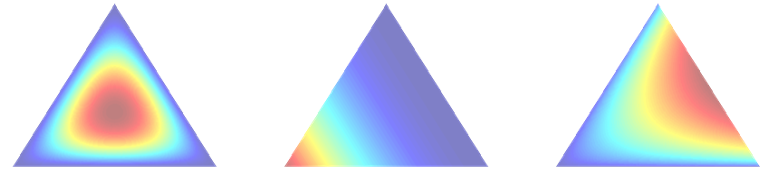
\includegraphics[width=\textwidth]{dirichlet.png}

\end{frame}

\subsection{Normal-gamma distribution}

\begin{frame}{Normal-gamma distribution}

\itemb
\item Normal (Gaussian) and Normal-gamma distributions
 \itemb
 \item Mean $\mu$, precision $\tau$ (precision is reciprocal of variance). \\
Data $\{x_i\}$ with moments $m_k = \sum_i x_i^k$
\begin{eqnarray*}
P({\bf x}|\mu,\tau)
& = & \prod_i \sqrt{\frac{\tau}{2\pi}} \exp \left( -\frac{\tau}{2}(x_i-\mu)^2 \right) \\
& = & \left(\frac{\tau}{2\pi}\right)^{m_0/2} \exp \left( -\frac{\tau}{2} (m_2 - 2\mu m_1 + \mu^2 m_0) \right)
\end{eqnarray*}
\iteme
\iteme

\end{frame}

\begin{frame}{Normal-gamma distribution}

\itemb
\item Normal
\[
P({\bf x}|\mu,\tau)
= \left(\frac{\tau}{2\pi}\right)^{m_0/2} \exp \left( -\frac{\tau}{2} (m_2 - 2\mu m_1 + \mu^2 m_0) \right)
\]
 \item Conjugate prior
\begin{eqnarray*}
P(\mu,\tau) & = & P(\tau) P(\mu|\tau) \\
P(\tau) & = & \frac{e^{-\beta \tau} \tau^{\alpha-1} \beta^\alpha}{\Gamma(\alpha)} \\
P(\mu|\tau) & = & \sqrt{\frac{\lambda \tau}{2\pi}} \exp\left( -\frac{\lambda \tau}{2}(\mu-\epsilon)^2 \right)
\end{eqnarray*}
\item $P(\tau)$ is gamma (shape $\alpha$, rate $\beta$)
\item $P(\mu|\tau)$ is Normal (mean $\epsilon$, precision $\lambda \tau$)
\item Full set of hyperparameters is $\{ \alpha, \beta, \epsilon, \lambda \}$
\iteme

\end{frame}

\begin{frame}{Normal-gamma distribution}

\itemb
\item Conjugacy:
\begin{eqnarray*}
P({\bf x}) & = & (2\pi)^{-m_0/2} \frac{\Gamma(\alpha')}{\Gamma(\alpha)} \frac{\beta^\alpha}{{\beta'}^{\alpha'}} \sqrt{\frac{\lambda}{\lambda'}} \\
P(\mu,\tau|{\bf x}) & = & 
\frac{e^{-\beta' \tau} \tau^{\alpha'-1} {\beta'}^{\alpha'}}{\Gamma(\alpha')} \times
\sqrt{\frac{\lambda' \tau}{2\pi}} \exp\left( -\frac{\lambda' \tau}{2}(\mu-\epsilon')^2 \right)
\end{eqnarray*}

where
$\epsilon' = \frac{\lambda\epsilon + m_1}{\lambda + m_0}$,
$\lambda' = \lambda + m_0$,
$\alpha' = \alpha + \frac{m_0}{2}$ and
$\beta' = \beta + \frac{1}{2}\left( \epsilon^2 + m_2 - \frac{(\lambda\epsilon + m_1)^2}{\lambda + m_0} \right)$.
\item NB if we regard $\tau$ as fixed, then Gaussian is auto-conjugate.
\iteme

\end{frame}

\begin{frame}{$\chi^2$ distribution}

\[
P(\mu,\tau|{\bf x}) = 
\frac{e^{-\beta' \tau} \tau^{\alpha'-1} {\beta'}^{\alpha'}}{\Gamma(\alpha')} \times
\sqrt{\frac{\lambda' \tau}{2\pi}} \exp\left( -\frac{\lambda' \tau}{2}(\mu-\epsilon')^2 \right)
\]

\itemb
\item Rescale the posterior distribution for $\tau$:
divide by $(m_2/m_0 - m_1^2/m_0)^{-1}$
(the posterior mean estimate for $\tau$)
\item Resulting gamma distribution with shape $m_0/2$ and scale $1/2$
is the ``$\chi^2$ distribution''.
\item Canonical definition of the quantity $\chi^2$
is in the special case where $\mu=0$ and $\tau=1$,
in which case $\chi^2=m_2$
\iteme

\end{frame}

\subsection{Summary}

\begin{frame}{Common conjugacies}

\itemb
\item Exponential/Poisson $\leftrightarrow$ Gamma
\item Binomial $\leftrightarrow$ Beta
\item Multinomial $\leftrightarrow$ Dirichlet
\item Normal $\leftrightarrow$ Normal-gamma
\iteme

\end{frame}


\section{MCMC in theory}

\subsection{Motivation}

\begin{frame}{Motivation}

\begin{tabular}{lr}
\Tree [ .$x_1$ [ .$x_2$ $y_4$ $y_5$ ] [ .$x_3$ $y_6$ $y_7$ ] ]
&
$P(X|Y) = \frac{P(X,Y)}{P(Y)} = \frac{P(X,Y)}{\sum_{X'} P(X',Y)}$
\end{tabular}

\itemb
\item Let $A$ = alphabet size
\item Felsenstein's pruning algorithm for $P(Y)$
 \itemb
 \item Time ${\cal O}(NA^2)$
 \item Memory ${\cal O}(NA)$
 \iteme
\item Exponentiating an $A \times A$ matrix $N$ times
 \inone{Time ${\cal O}(NA^3)$}
\item OK: bases ($A=4$), amino acids ($A=20$), codons ($A=64$)
\itemb
\item Painful: Gene Ontology ($A=33,587$), GO-Slim ($A=127$)
\iteme
\iteme

\end{frame}


\begin{frame}{MCMC: general idea}

\itemb
\item Want to sample from some pdf $P(X) = \frac{f(X)}{Z}$ where $X \in {\cal X}$
\item Problem: set ${\cal X}$ is large; computing $Z = \sum_{X \in {\cal X}} f(X)$ is hard
\item Construct a stochastic process $X_1, X_2, X_3, X_4, \ldots$
such that the equilibrium distribution is $P(X)$
\item If the process is ergodic, then $X_t \sim P(X)$ for ``large'' $t$
\inone{How large must $t$ be? The \alert{burn-in time} or \alert{mixing time}}
\iteme

\end{frame}


\begin{frame}{MCMC: construction}

\itemb
\item Want a Markov process $X_1, X_2, \ldots$ w/equilibrium $P(X)$
\item Let $Q(i,j) = P(X_{t+1}=j | X_t = i)$  be the \alert{transition matrix}
\item One way to make $P(X)$ the equilibrium distribution is to force $Q$ to satisfy \alert{detailed balance}
\[
P(i) Q(i,j) = P(j) Q(j,i) \quad \quad \forall i,j \in {\cal X}
\]
\item If $P(X) = \frac{f(X)}{Z}$ we can drop the $Z$
\[
f(i) Q(i,j) = f(j) Q(j,i)
\]
\item Note this process is \alert{reversible} (MCMC doesn't have to be, but usually is)
\iteme

\end{frame}

\subsection{Metropolis-Hastings}

\begin{frame}{Metropolis-Hastings algorithm: the proposal}

\itemb
\item One way to construct a $Q$ that satisfies detailed balance
\[
f(i) Q(i,j) = f(j) Q(j,i)
\]
\item Start with a \alert{proposal distribution} $U(i,j) = P(X_{t+1}=j|X_t=i)$
 \itemb
 \item Metropolis/Teller (1953): \alert{symmetric} proposal, $U(i,j)=U(j,i)$
 \item Hastings (1970) generalized to \alert{reversible} proposal
\[
g(i)U(i,j)=g(j)U(j,i)
\]
 \item Note $g \neq f$: proposal does {\bf not} have to converge on $f$
 \iteme
\item Now we adapt this $U$ to construct $Q$
\iteme

\end{frame}


\begin{frame}{Metropolis-Hastings algorithm: accept/reject}

\itemb
\item We have a proposal density, $U$, satisfying (for some $g$)
\[
g(i)U(i,j)=g(j)U(j,i)
\]
\item Process:
 \itemb
 \item Given $X_n$, \alert{propose a move} by sampling $X'$ from
\[
P(X'=j|X_n=i) = U(i,j)
\]
 \item Calculate the \alert{Hastings ratio}
\[
h(X,X') = \frac{f(X')}{f(X)} \frac{g(X)}{g(X')} = \frac{f(X')}{f(X)} \frac{U(X',X)}{U(X,X')}
\]
 \item If $h(X,X') \geq 1$, then \alert{accept the move}: set $X_{n+1} \leftarrow X'$
 \item If $h(X,X') < 1$, then
  \itemb
  \item Sample an r.v. $\alpha$ from $U(0,1)$ (uniform distribution)
  \item If $\alpha < h(X,X')$, then accept the move
  \item If $\alpha \geq h(X,X')$, then \alert{reject the move}: set $X_{n+1} \leftarrow X_n$
  \iteme
 \iteme
\iteme

\end{frame}


\begin{frame}{Metropolis-Hastings: proof of detailed balance}

\begin{eqnarray*}
h(i,j) & = & \frac{f(j)}{f(i)} \frac{U(j,i)}{U(i,j)} \\
Q(i,j) & = & U(i,j) \times \min\left( 1, h(i,j) \right)
\end{eqnarray*}

\itemb
\item Suppose (with no loss of generality) that $h(i,j) \leq 1$
\begin{eqnarray*}
Q(i,j) & = & U(i,j) h(i,j) \\
& = & U(i,j) \frac{f(j)}{f(i)} \frac{U(j,i)}{U(i,j)} \\
& = & \frac{f(j)}{f(i)} U(j,i)
\end{eqnarray*}
\item Since $h(j,i) \geq 1$, we must have $Q(j,i) = U(j,i)$, and so
\[
f(i) Q(i,j) = f(j) Q(j,i)
\]

\iteme

\end{frame}


\subsection{Gibbs sampling}

\begin{frame}{Gibbs sampling}

\Tree [ .$x_1$ [ .$x_2$ $y_4$ $y_5$ ] [ .$x_3$ $y_6$ $y_7$ ] ]

\itemb
\item The $X$ in $P(X)$ is $N$-dimensional, $X = (x_1,x_2 \ldots x_N)$
\item \alert{Gibbs Sampling} proposal distribution is as follows
 \itemb
 \item Pick a dimension $m$, where $1 \leq m \leq N$
 \item Conceptually, fix all of the $\{x_n\}$ except for $x_m$; sample $x_m$ from its marginal distribution conditional on all the others
 \item Proposal distribution is
\begin{eqnarray*}
U(X,X') & = & U(\{x_n\},\{x'_n\}) \\
& = & P(x'_m | \{x_n:n \neq m\}) \times \prod_{n \neq m} \delta(x'_n = x_m)
\end{eqnarray*}
 \iteme
 \item All proposals accepted: Hastings ratio always 1 (\alert{prove it!})
\iteme

\end{frame}


\begin{frame}{Gibbs sampling: the marginal distribution}

Let $X_{\mbox{other}} = \{x_n:n \neq m\}$

\begin{eqnarray*}
P(x'_m | X_{\mbox{other}}) & = & \frac{P(x'_m, X_{\mbox{other}})}{P(X_{\mbox{other}})} \\
& = & \frac{P(x'_m, X_{\mbox{other}})}{\sum_k P(x'_m = k, X_{\mbox{other}})} \\
\end{eqnarray*}

If $P(X)$ is a product of functions of sparse subsets of $X$ (c.f. factor graphs),
then many of these functions will cancel in numerator and denominator

\end{frame}

\begin{frame}{Gibbs sampling: factor graph example}

\small
\Tree [ .$f_1$ [ .$x_1$
 [ .$f_2$ [ .\alert{$x_2$} [ .$f_4$ [ .$x_4$ $f_{4a}$ ] ] [ .$f_5$ [ .$x_5$ $f_{5a}$ ] ] ] ]
 [ .$f_3$ [ .$x_3$ [ .$f_6$ [ .$x_6$ $f_{6a}$ ] ] [ .$f_7$ [ .$x_7$ $f_{7a}$ ] ] ] ]
] ]

\vspace{\baselineskip}

\normalsize
\[
P(x'_2|X_{\mbox{other}}) = \frac{f_2(x_1,x'_2) f_4(x'_2,x_4) f_5(x'_2,x_5)} {\sum_k f_2(x_1,k) f_4(k,x_4) f_5(k,x_5)}
\]

\end{frame}


\begin{frame}{Interlude: the Jacobian matrix and its determinant}

\itemb
\item Function $F:\Re^n \to \Re^m$
\item Let $(y_1 \ldots y_m) = F(x_1 \ldots x_n)$
\item The \alert{Jacobian matrix} of $F$ is
\[
J_F(x_1,\ldots,x_n) =
\begin{bmatrix} \dfrac{\partial y_1}{\partial x_1} & \cdots & \dfrac{\partial y_1}{\partial x_n} \\ \vdots & \ddots & \vdots \\ \dfrac{\partial y_m}{\partial x_1} & \cdots & \dfrac{\partial y_m}{\partial x_n}  \end{bmatrix}
\]
\item For square matrices ($m=n$), the magnitude of the \alert{Jacobian determinant}, $|\mbox{det}(J_F)|$, gives the factor by which the function $F$ expands or shrinks volumes in ${\bf x}$
\iteme

\end{frame}

\begin{frame}{Interlude: multidimensional change of variables}

\itemb
 \item If $p(x)$ is pdf of $x$, and $y=F(x)$, what is pdf $q(y)$ of $y$?
  \inone{Now with multidimensional $x=(x_1\ldots x_n)$ and $y=(y_1 \ldots y_n)$ }
 \item Derivation:
\begin{eqnarray*}
dy_1 dy_2 \ldots dy_n & = & \left|\mbox{det}\left(J_F\right)\right| dx_1 dx_2 \ldots dx_n \\
q(y) dy_1 dy_2 \ldots dy_n & = & p(x) dx_1 dx_2 \ldots dx_n \\
q(y) & = & p(x) / \left|\mbox{det}\left(J_F\right)\right| \\
& = & p(F^{-1}(y)) \left|\mbox{det}\left(J_{F^{-1}}\right)\right|
\end{eqnarray*}
where the last line uses the \alert{inverse function theorem},
\[
J_{F^{-1}} = \left( J_F \right)^{-1}
 \quad \quad \mbox{... c.f. \alert{chain rule}: $J_{F \circ G}(x) = J_F(G(x)) J_G(x)$}
\]
\iteme

\end{frame}


\begin{frame}{MCMC on continuous variables}

\itemb
\item Let $x$ be a continuous state
\item Suppose the proposal generates $x'$ by sampling some parameter $u$ from a p.d.f. $g(u)$, so $x'=x'(x,u)$
\itemb
 \item Let $u'=u'(x,u)$ be the \alert{inverse} parameter that takes us back from $x' \to x$
 \item For convenience, define the function $F(x,u) = (x',u')$
\iteme
\item The Hastings ratio then depends on the Jacobian $J_F$
\[
h(x,x') = \frac{P(x')}{P(x)} \frac{g(u')}{g(u)} \left| \mbox{det}\left(J_F\right) \right|
\]
\item Interpretation: we are moving through $(x,u)$-space rather than just $x$-space
%\alert{Think about this some more!}
\item Green (1995, 2003)
\iteme

\end{frame}



\begin{frame}{There's more}

\itemb
\item Summarizing results of an MCMC run
\item Diagnosing MCMC convergence
\itemb
\item Replicates
\item Intra- and inter-chain variance
\iteme
\iteme
\end{frame}


\section{MCMC in bioinformatics}

\begin{frame}{Sampling ungapped sequence alignments}

\itemb
\item Example: ungapped sequence alignments (Lawrence {\em et al})
 \itemb
 \item Suppose you have $K$ sequences, $\{ S^{(1)} \ldots S^{(K)} \}$, and that $S^{(k)}_i$ is the $i$'th residue of the $k$'th sequence.
 \item Let $x_k$ be the indentation of the $k$'th sequence. The motif (of length $M$) runs from $x_k$ to $x_k+M-1$.
 \iteme
\iteme

\end{frame}


\begin{frame}{Sampling ungapped alignments}

\itemb
 \item Let ${\cal U}$ denote the null hypothesis that the sequences are unrelated. Then
\[
\frac{P({\bf x})}{P({\cal U})} = \prod_{m=0}^{M-1} \frac{f({\bf n}(m))}{\prod_\omega q(\omega)^{n_\omega(m)}}
\]
where $q(\omega)$ is a background distribution over alphabet symbols $\omega$, and $n_{\omega}(m)$ is the number of times symbol $\omega$ appears in column $m$ of the motif
\[
n_{\omega}(m) = \sum_{k=1}^K \delta(S_{x_k + m} = \omega)
\]
\iteme

\end{frame}


\begin{frame}{Sampling ungapped alignments}

\itemb
\item The $f({\bf n})$ function should reward conserved columns.
Lawrence {\em et al} use an entropy-like measure
\[
f({\bf n}) = \prod_\omega p_\omega^{n_\omega} = \exp (-KS[p])
\]
where $p_k = n_k/K$.
Note that this is the distribution ${\bf p}$ that maximizes $\prod_\omega p_\omega^{n_\omega}$ for a given ${\bf n}$.
Due to this implicit maximization, the above $f({\bf n})$ is not strictly a probability distribution for ${\bf n}$.
 \item Typically a vector of pseudocounts ${\bf a}$ is added to ${\bf n}$.
This suggests the Dirichlet evidence as an alternative form for $f$ that does not involve any implicit maximization:
\[
f({\bf n}) = \frac{{\cal B}({\bf n} + {\bf a})}{{\cal B}({\bf a}){\cal B}({\bf n})}
\]
\iteme

\end{frame}


\begin{frame}{Sampling ungapped alignments}

\itemb
 \item Another way to formulate this problem is as a chain over $({\bf x},\{{\bf p}(m)\})$ with Gibbs-sampling steps that alternate between resampling one of the $x_k$'s and resampling all the ${\bf p}$'s.
 \item For good mixing it's also useful to allow moves that slide the entire motif window, i.e. ${\bf x} \leftarrow {\bf x} \pm {\bf 1}$
\iteme

\end{frame}


\begin{frame}{Sampling ungapped alignments}

\itemb
 \item Sometimes you want to sample over the motif width $M$ as well.
  \itemb
  \item Consider however the following subtlety that arises if you keep track of the position-specific probabilities as part of the chain (instead of using the Dirichlet-evidence approach).
  \item If the chain state is $({\bf x},M,{\bf p}(1) \ldots {\bf p}(M))$ and you move from $M \to M+1$,
then you need a new vector of probabilities ${\bf p}(M+1)$ and so the dimensionality of your state space has changed, which is a Bad Thing for reversibility.
  \item The idea of \alert{reversible jump MCMC} is to set a ceiling for $M$ (let's say $M_{\max}$) and to let the state be $({\bf x},M,{\bf p}(1) \ldots {\bf p}(M_{\max}))$.
  \item For a particular $M < M_{\max}$, the parameters ${\bf p}(M+1) \ldots {\bf p}(M_{\max})$ are unused ``dummy'' parameters that are simply there to pad out your ``real'' parameters,
so that the dimensionality of your state space is fixed.
  \iteme
 \iteme

\end{frame}




\end{document}
